\section{Analysis Procedure} \label{sec:ana}
% \begin{flushleft}
    \subsection{Analysis overview}
Our goal is to find the axion signal hidden in the white noise. In order to achieve this, our analysis procedure includes the following steps:
    \begin{enumerate}
        %\item Read raw data (I, Q) from tdms file and do Fast Fourier transform every 1 millisecond of spectrum, then average all over spectra in 1 second to get power spectrum.
        \item Perform Fast Fourier transform (FFT) time-dependent spectrum to obtain the frequency-dependent spectrum.
        %\item Divide the measured power by the gains from the receiver chain to retrieve real power from cavity.
        %\item HEMT drift to predict noise and gain from the environmental parameters.
        %\item Use the results of high-electron-mobility-transistor(HEMT) drifting (see Section \ref{hemt_drifting}) to predict adding noise and gain; the input environmental parameters include monitoring temperatures, voltages of power supplies, etc.
        %\item Use Savitzky-Golay filter \cite{SGFilter} to remove the spectrum structure, then subtract the mean power.
        \item Apply Savitzky-Golay (SG) filter to the oscillating structure of the frequency-dependent spectrum
        \item Combine all power spectra from different frequency scans with weighting algorithm.
        %\item Cause the expected Axion bandwidth, and our frequency resolution is 1KHz, so we need to merge the bin.
        \item Merge bins in the combined spectrum to maximize the SNR.
        %\item Set threshold at ${3.355\ \sigma}$.
        \item Set limit on \gagg.
    \end{enumerate}

    The analysis was done by closely following the procedure from the Haystac experiment ~\cite{HAYSTACII}.
% \end{flushleft}

%\subsection{Tdms}
\subsection{Fast Fourier transform}
%For each frequency scan, we collected data for 12.5 hours. The recorded data were stored in TDMS files (Technical Data Management Streaming - binary file format developed by \textbf{National Instruments}). Each TDMS file contains 2 millions data points corresponding to 1000 time dependent subspectra. We performed Fast Fourier Transform (FFT) on each subspectrum to get the power in frequency (Eq.\ref{eq:4.1}).The I and Q in Eq.\ref{eq:4.1} are the raw data in voltage, R (50 Ohms) is the resistor of the signal analyzer, and 2000 is the number of data points. Finally, we averaged every 1000 successive subspectra to obtain the mean power in one second.
The time-dependent I and Q data were recorded and saved in TDMS (Technical Data Management Streaming) files - binary format developed by \textbf{National Instruments}.
%Fast Fourier Transform (FFT) was performed to convert the data into frequency-dependent and into unit of power by using the equation:
Fast Fourier Transform (FFT) was performed to convert the data into frequency-dependent from which power was calculated by using the equation:

\begin{equation}
\label{eq:4.1}
    \text{Power} = \frac{|\text{FFT}(I+i \cdot Q)|^{2}}{N \cdot 2R}
\end{equation}

where N is the number of data points ($N_A $ = 2000 in our experiment), and R is the resistance of the signal analyzer (50 $\Omega$).
The FFT was done for every one-second subspectrum data.

%\subsection{Gain}
%The net gain of our receiver chain includes: down conversion gain, Intermediate Frequency(IF)  attenuator, Radio Frequency(RF) attenuator and HEMT gain. The first three were the parameters set during data taking, the last one was estimated from calibration (Section \ref{sec:}). Fig.\ref{fig:Hemt_gain} shows the gain and noise from the HEMT calibration done before the data run.
%\newline
%After removing all the gains, we got the real power going out from the antenna of the cavity. The variation of the real power in time is shown in Fig. \ref{fig:over_temp}. One possible cause of this effect came from the additional gain variation that was not studied in the initial HEMT calibration before taking data. To investigate this issue, we did HEMT drifting to check the behaviour of the gain over time.

%\begin{figure}[h]
%    \centering
%%    \includegraphics[width=0.4\textwidth,height = 0.25\textwidth]{Figure/CD099_HEMT.jpg}
%    \caption{ Gain and noise of HEMT before running data}
%    \label{fig:Hemt_gain}
%\end{figure}
%\begin{figure}[h]
%\centering
% %   \includegraphics[width=0.4\textwidth,height=4cm]{Figure/overall_temp.png}
%    \caption{Power over the time from step 1 to step 16}
%    \label{fig:over_temp}
%\end{figure}
%} // comment the paragraph of gain
%%\newpage


%\begin{figure}
%     \begin{subfigure}[b]{.24\textwidth}
%       \centering
%        \includegraphics[width=\linewidth,height=3cm]{Figure/before_sg.png}
%        \caption{Before SG filter}
%        \label{fig:before_sg}
%    \end{subfigure}%
%    \hfill
%    \begin{subfigure}[b]{.24\textwidth}
%        \centering
%        \includegraphics[width=\linewidth,height=3cm]{Figure/sg_result.png}
%        \caption{SG filter}
%        % \caption{Raw power of 1s data (blue line) and the output Savitzky-Golay filter (red line)}
%        \label{fig:sg_result}
%    \end{subfigure}%
%    \vskip\baselineskip
%    \begin{subfigure}[b]{.24\textwidth}
%        \centering
%        \includegraphics[width=\linewidth,height=3cm]{Figure/After_Sg.png}
%        \caption{After SG filter}
%        \label{fig:After_Sg}
%    \end{subfigure}%
%    \hfill
%    \begin{subfigure}[b]{.24\textwidth}
%        \centering
%        \includegraphics[width=\linewidth,height=3cm]{Figure/system_temp.png}
%        \caption{System temperature}
%        \label{fig:system_temp}
%    \end{subfigure}%
%    \caption{\textbf{(a)} The power spectra after average 12.5 hours of data. \textbf{(b)} Raw power of 1s data (blue line) and the output Savitzky-Golay filter (red line). \textbf{(c)} After dividing the sg filter's result in every step \textbf{(d)} The system temperature derived from $\mu$ and $\sigma$. }
    % \label{fig:fig}
%\end{figure}

% \begin{center}
% \begin{figure*}[!tbp]
% \centering
%     \begin{minipage}[t]{.24\textwidth}
%     \centering
%     \includegraphics[width=1\textwidth,
%     height = 0.75\textwidth]{Figure/before_sg.png}
%     \caption{Before SG filter}
%     \label{fig:before_sg}
%     \end{minipage}%
%     \hfill
%     \begin{minipage}[t]{.24\textwidth}
%     \centering
%     \includegraphics[width=1\textwidth,
%     height = 0.75\textwidth]{Figure/After_Sg.png}
%     \caption{After SG filter}
%     \label{fig:After_Sg}
%     \end{minipage}%
%     \hfill
%     \begin{minipage}[t]{.25\textwidth}
%     \centering
%     \includegraphics[width=1\textwidth,
%     height = 0.75\textwidth]{Figure/system_temp.png}
%     \caption{The system temperature calculate by $\mu$ and $\sigma$}
%     \label{fig:system_temp}
%     \end{minipage}%
% \end{figure*}
% \end{center}


%\subsection{Savitzky Golay filter}
\subsection{Remove the oscillating structure}
%Figure \ref{fig:sg_result} is the spectrum in each step, somehow they all have a similar structure, in order to remove this structure, we will use a Savitzky Golay filter in every second to smooth the data Figure \ref{fig:After_Sg}.

In case of absence axion signal, the output data is the noise of the cavity and the amplification chain. If axion presents in the cavity, its power will be buried in the noise because the signal is very weak. Therefore, the structure of the raw output power spectrum, as shown in Fig.~\ref{fig:raw_sg_power}, is the product of the noise and the gain of the system. The Savitzky Golay (SG) filter ~\cite{SGFilter}, a digital filter that can smooth data without distorting the signal tendency, was applied to remove the structure or background.
The filter was performed on average spectrum of each scan by fitting adjacent points of successive sub-sets of data with a nth-order polynomial. The result depends on two parameters: the number of data points used for fitting, so-called the window width, and the order of the polynomial. If the window is too wide, the filter will not remove small structures and if it is too narrow, it may kill the signal. The window and order were first chosen during the data taking based on the structure of data and the ratio between raw data and the filter output. After data taking, they were optimized by injecting axion signal on top of noise data and found that they were consistent with the first choice.
The raw average spectrum was divided by the output of the SG filter and subtracted by 1 to get normalized spectrum (Fig.~\ref{fig:raw_sg_power}).
Therefore, if the axion signal exists, the excess power will be above 0.
%After filtering, the normalized spectrum (Fig. \cite{fig:}) was obtained by dividing the raw spectrum by the output of the SG filter subtract 1. Therefore, if the signal exists, the excess power will be above 0.
Since we adjusted the resonant frequency of the cavity to scan large range and to reduce the noise at overlapped region, we need to combine all the spectra of all scans to create one big spectrum. Before doing this, the normalized spectrum from each scan was rescaled by the system noise [detailed in Sec~\ref{sec:calibration}] and the signal power with taking the cavity Lorentzian shape into account. The rescaled spectrum, shown in Fig.~\ref{res_spectrum}, was computed with formula:

\begin{equation}
  \label{eq:respower_eqn}
  \delta_{ij}^{res} = \frac{k_{B}T_{sys}\Delta\nu \delta_{ij}^{norm}}{P_{ij}^{s} h}
\end{equation}

and standard deviation of each bin is:
\begin{equation}
  \label{eq:ressigma_eqn}
  \sigma_{ij}^{res} = \frac{k_{B}T_{sys}\Delta\nu \sigma_{i}^{norm}}{P_{ij}^{s} h}
\end{equation}

where $\delta_{ij}^{norm}$ and $\sigma_{i}^{norm}$ are the power and the standard deviation of
bin $j^{th}$ from the normalized spectrum $i^{th}$,
$\Delta\nu$ is the bin width of spectrum, $P_{ij}^{s}$ is the KSVZ axion signal power,
and $h = \frac{1}{1 + [2(\nu_{ij} - \nu_{ci})/\Delta\nu_{i}]}$ is Lorentzian shape of the cavity,
$\Delta\nu_{i}$ is the cavity line width which depends on the resonant frequency and the intrinsic quality factor.

If a signal appears in a certain frequency bin $j^{th}$, its expected power will be enhanced or reduced depending on the bin position due to the cavity's Lorentzian shape. The rescaling will take into account this effect.

\begin{figure} [htbp]
  \centering
  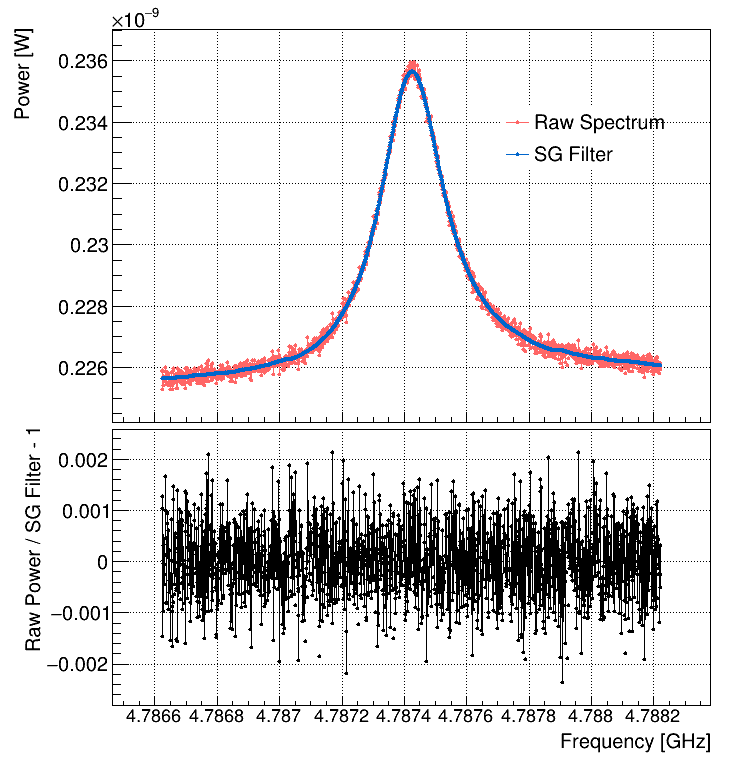
\includegraphics[width=0.38\textwidth,height = 0.4\textwidth]{figures/RawPower_SGPower_Ratio_vs_Freq_Step_0100.png}
  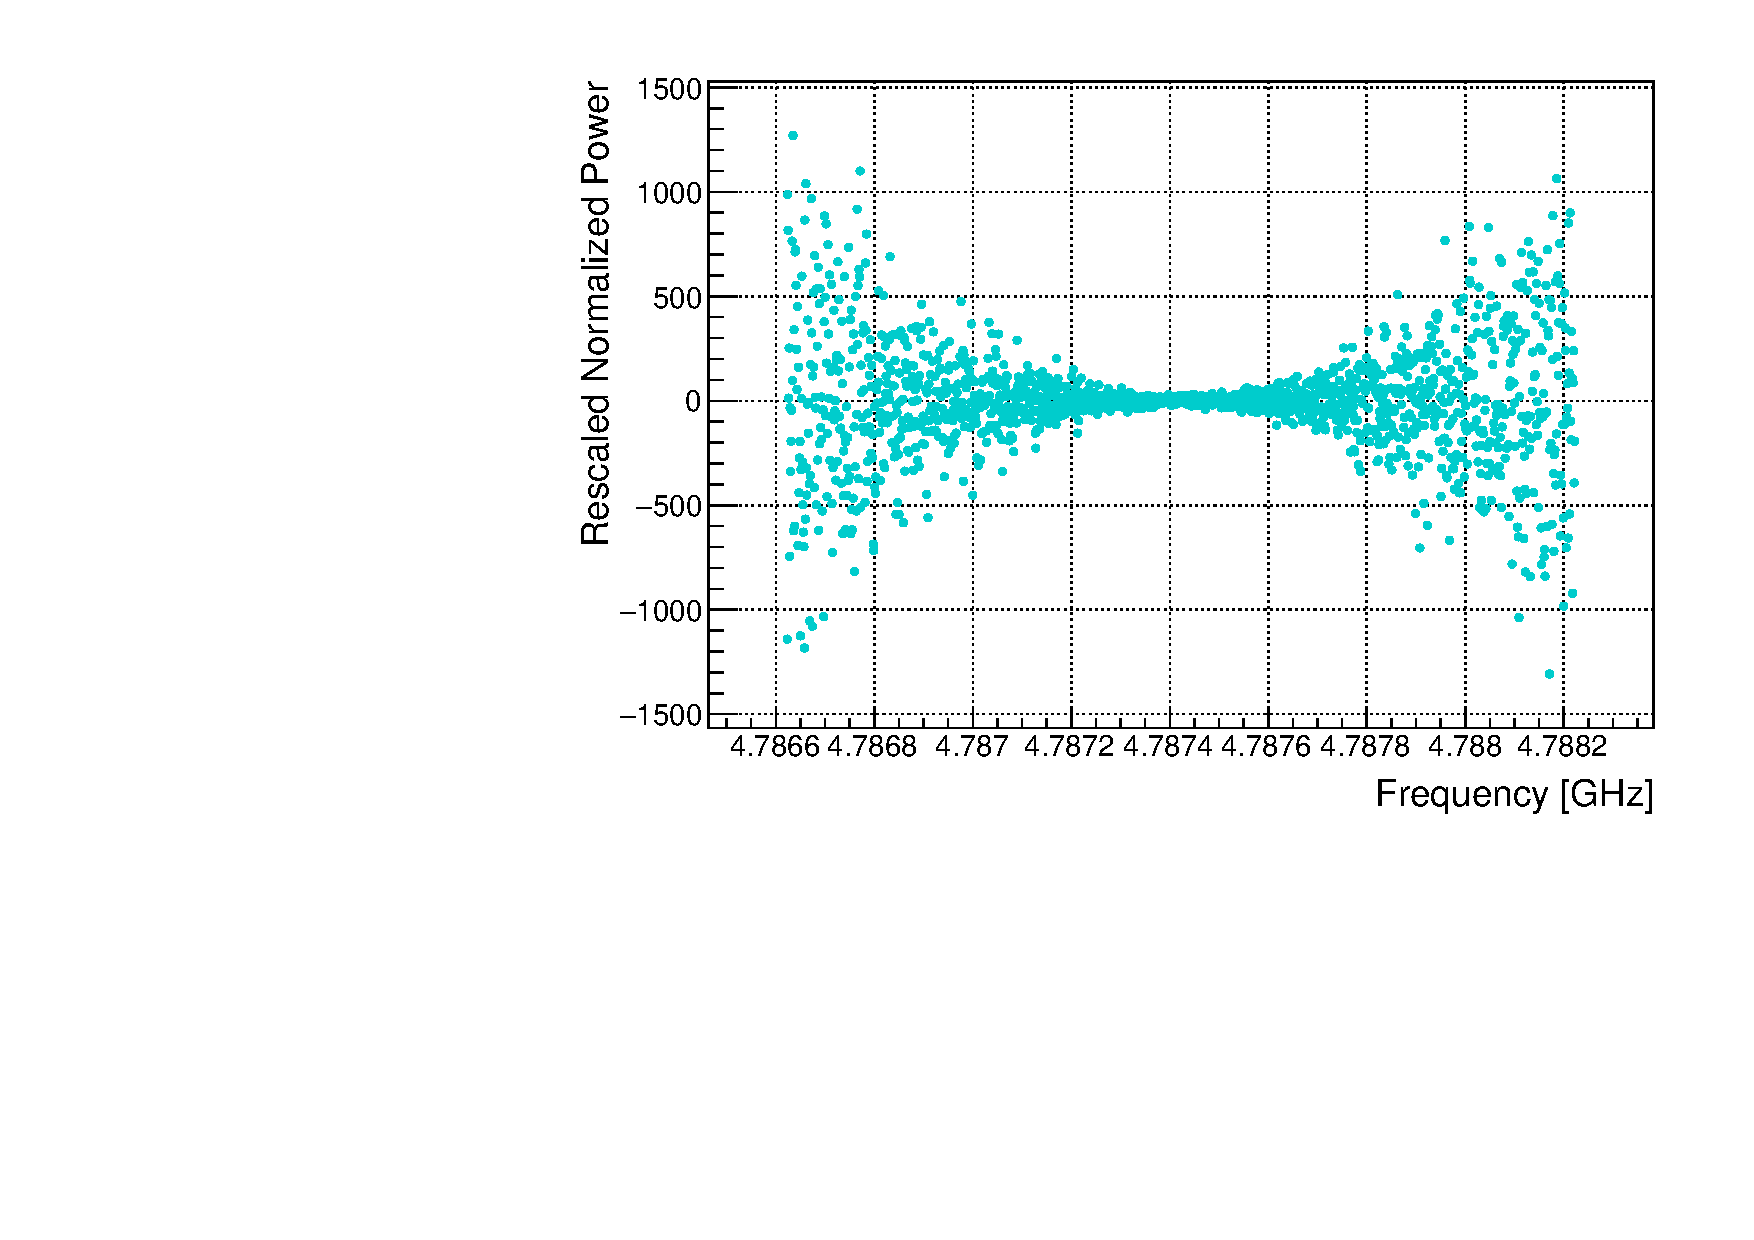
\includegraphics[width=0.52\textwidth,height = 0.4\textwidth]{figures/RescaledPower_vs_Freq_Step_0100.pdf}
  \caption{Left: Upper panel: Raw power spectrum (blue) and output of SG filter (red) of one scan. Bottom panel: Rescaled spectrum derived by the ratio of the raw spectrum and the SG fitler in the left and subtract 1.
  Right: Rescaled power spectrum obtained by multiplying the normalized power with system noise and dividing expected axion signal power taking the Lorentzian shape of cavity into account}
  \label{fig:raw_sg_power}
\end{figure}

%\begin{figure} [htbp]
%  \centering
%  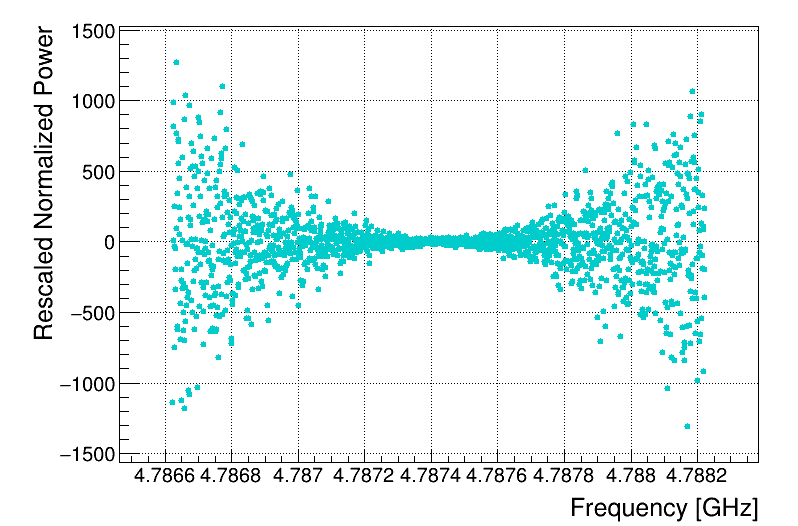
\includegraphics[width=0.4\textwidth,height = 0.4\textwidth]{figures/RescaledPower_vs_Freq_Step_0100.png}
%  \caption{Rescaled power spectrum obtained by multiplying the normalized power with system noise and dividing expected axion signal power% taking the Lorentzian shape of cavity into account}
%  \label{fig:res_spectrum}
%\end{figure}



%First we will choose a window and a order, then move the window and fit the data a with a polynomial with chosen order, it is a kind of generalization  moving average characterized, if the windows is too big, then it will not remove small structures, if it too small, it may kill the signal, you can see that choosing an appropriate window is important, a way to test if the windows are appropriate is to see the system temperature calculated by  $\mu$ and $\sigma$.

%\begin{equation}
%    \label{eq:ts_mu}
%    \mu = k_{B} \cdot T_{S} \cdot \Delta \nu 
%\end{equation}
%\begin{equation}
%    \label{eq:ts_sigma}
%    \sigma = \frac{k_{B} \cdot T_{S} \cdot \Delta \nu}{\sqrt{N}}
%\end{equation}

%If we treat the spectrum after the SG filter as a pure noise, we know that the system temperature of a white noise can be calculated by $\mu$ and $\sigma$ (Eq.\eqref{eq:ts_mu}) (Eq.\eqref{eq:ts_sigma}),
%where $k_{B}$ is the Boltzmann constant, $T_{S}$ is the system temperature, $\Delta \nu$ is the frequency resolution and N is the number of averaging. \\
%If the chosen window is appropriate, the system temperature estimated from $\mu$ and $\sigma$ should be consistent  with each other. \\

%We also did some studies to check if the SG filter removed the axion signal. Assuming a signal bandwidth of 5 kHz, we added the signal into noise spectrum and applied the SG filter. The result shows that the filter does not suppress the axion signal as given in Fig.\ref{fig:weighted_snr}.

%about whether the sg filter will remove the Axion signal, assuming the Axion signal bandwidth is 5KHz, add the signal in a white noise and apply the sg filter , the results show that it will not affect much before and after use, after divide the sg filter result, we will subtract 1 to make the value become 1.

%\begin{figure}[h]
%    \begin{minipage}[h]{.5\textwidth}
%    \centering
%    \includegraphics[width=0.8\textwidth, height = 0.5\textwidth]{Figure/sg_simulation.png}
%    \caption{The simulation for testing the effect of SG filter.}
%    \label{fig:weighted_snr}
%%    \end{minipage}%
%\end{figure}
%\begin{figure}[h]
%    \begin{minipage}[t]{.5\textwidth}
%    \centering
%    \includegraphics[width=0.8\textwidth,height = 0.5\textwidth]{Figure/weighted_snr.png}
%    \caption{Weighed SNR}
%    \label{fig:weighted_snr}
%%    \end{minipage}%
%\end{figure}

\subsection{Combine spectra with weighting algorithm} \label{weighting_algorithm}

The purpose of weighting algorithm is to add different spectra vertically, particularly for the frequency bins that appear in multiple spectra.  %Each spectrum in Fig.\ref{fig:After_Sg}
Each spectrum was collected with a different cavity resonance frequency. Therefore, if a signal appears in a certain frequency bin $j^{th}$, due to the difference in resonance frequency and Lorentzian shape, the expected signal power will be different in each spectrum $i$. The weighting algorithm is expected to take this into account with weight calculated for each bin j of normalized spectrum i defined in Eq.\cite{eq:weight}.
The weighted power $\delta^{com}_{n}$ and standard deviation $\sigma^{com}_{n}$ of each bin $n$ in the combined spectrum are calculated using Eq.~\ref{eq:comb_power} and Eq.~\ref{eq:comb_sigma}, respectively. The SNR is the ratio of $\delta^{com}_{n}$ and $\sigma^{com}_{n}$ as given in Eq.~\ref{eq:comb_snr}.

%The purpose of weighting algorithm is to add different spectrum vertically, we have different spectrum with different resonance frequency Figure \ref{fig:After_Sg}, so we need a weight for add them up. Eq.\eqref{eq:weight}.

\begin{equation}
    \label{eq:weight}
    %    {w_{n}}^{i} = \frac{h \cdot p}{(\sigma_{n}^{i})^{2}}
    {w_{j}} = \frac{1}{(\sigma_{ij}^{res})^{2}}
\end{equation}

\begin{equation}
    \label{eq:comb_power}
    \delta_{n}^{com} = \frac{ \sum_{1}^{k}\delta_{ij}^{res} \cdot {w_{ij}}}{\sum_{1}^{k} {w_{ij}}}
\end{equation}
\begin{equation}
    \label{eq:comb_sigma}
    \sigma_{n}^{com} = \frac{ \sqrt{\sum_{1}^{k}(\sigma_{ij}^{res} \cdot {w_{ij}})^2}}{\sum_{1}^{k} {w_{ij}}}
\end{equation}
\begin{equation}
    \label{eq:comb_snr}
    {SNR}_{n}^{com} = \frac{\delta^{com}_{n}}{\sigma^{com}_{n}}= \frac{\sum_{1}^{k}\delta_{ij}^{res} \cdot {w_{ij}}^{res}}{ \sqrt{\sum_{1}^{k}(\sigma_{ij}^{res} \cdot {w_{ij}}^{res})^2}}
\end{equation}

with i running from 1 to k - number of spectra containing bin j.

\begin{figure}[h]
    \centering
    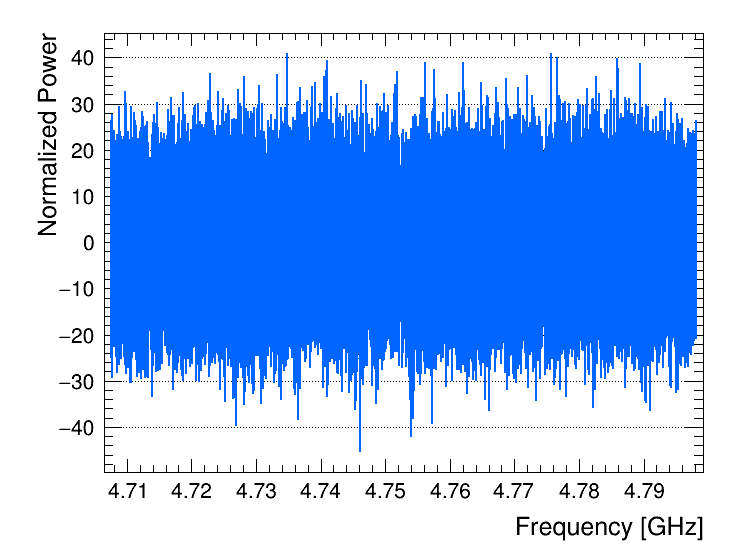
\includegraphics[width=0.4\textwidth,height = 0.3\textwidth]{figures/Power_CombSpectrum_AxionRun_AllSteps_Rescan_SG4_W201_LqWeight.png}
    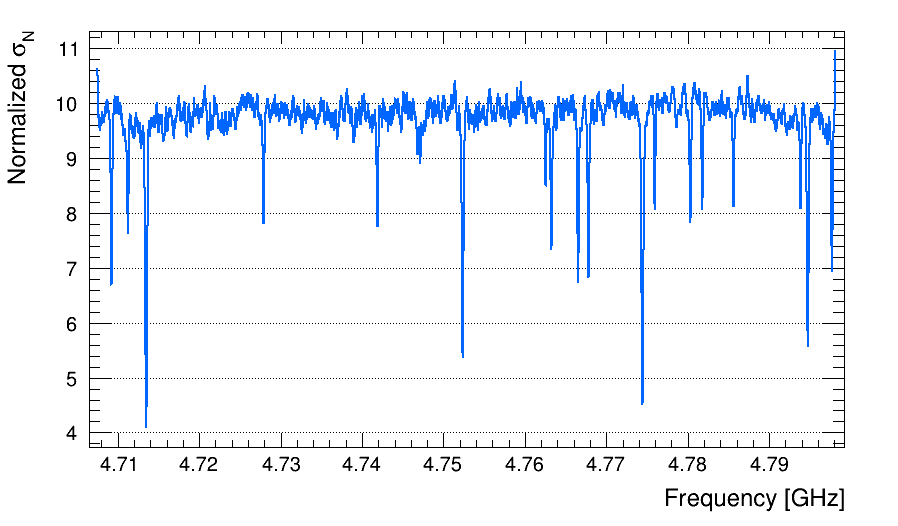
\includegraphics[width=0.4\textwidth,height = 0.3\textwidth]{figures/Sigma_CombSpectrum_AxionRun_AllSteps_Rescan_SG4_W201_LqWeight.png}
    \caption{The combined power $\delta$ following Eq.\eqref{eq:comb_power} (left) and the standard deviation $\sigma$ derived from Eq.\eqref{eq:comb_sigma} (right)}
    \label{fig:power_sigma_comb}
\end{figure}

\begin{figure}[hbt!]
    \centering
    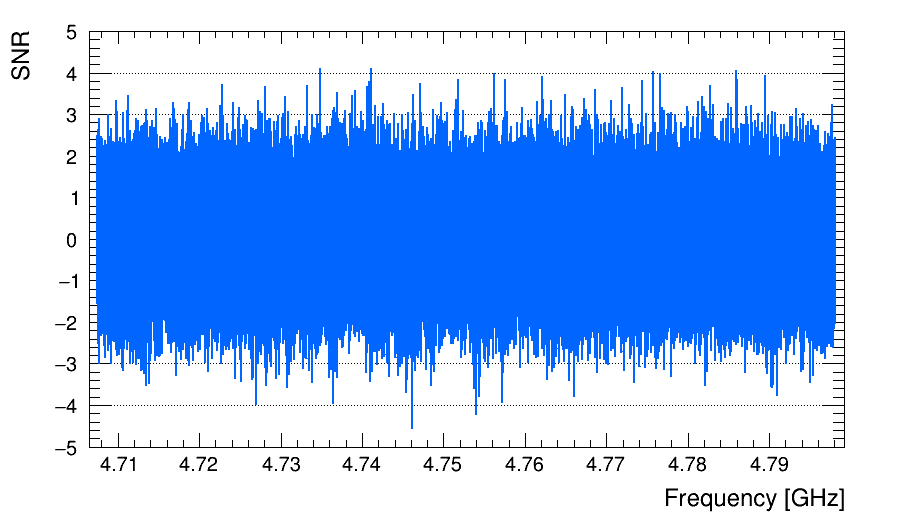
\includegraphics[width=0.8\textwidth,height=0.4\textwidth]{figures/SNR_CombSpectrum_AxionRun_AllSteps_Rescan_SG4_W201_LqWeight.png}
    \caption{Signal-to-noise ratio (SNR) calculated using Eq.\eqref{eq:comb_snr} of the combined spectrum }
    \label{fig:SNR_comb}
\end{figure}


%where ${\delta_n^i}$ and ${\sigma_n^i}$ are the measured power and the corresponding standard deviation of the ${n^{\mathrm{th}}}$ frequency bin of the ${i^{\mathrm{th}}}$ spectrum., From the weighted power in ${n^{th}}$ bin in Eq.\eqref{eq:weighted_power}, and weighted $\sigma$ in Eq.\eqref{eq:weighted_sigma}, we can get our Signal to noise ratio as Eq.\eqref{eq:weighted_SNR}

\subsection{Merging bins}

With the quality factor of $10^6$, the expected axion bandwidth is of 5 kHz at frequency of 5 GHz. In this paper, our interested range is 4.7 - 4.8 GHz and the bin width is of 1 kHz. Therefore, in order to maximize the SNR, we merged M = 5 consecutive bins with overlapping of the combined spectrum to construct a final spectrum.
The purpose of overlapping is to avoid the signal power broken into different neighbouring bins of the merged spectrum. Before defining weights for merging, we multiplied the power and standard deviation of each bin in the combined spectrum by M: $\delta^{c}_n \rightarrow M\delta^{com}_n$ and $\sigma^{c}_n \rightarrow M \sigma^{com}_n$. This rescaling gives the expected mean of the normalized power $\mu^{com}_k = 1$ if a KSVZ axion signal power leaves a fraction of 1/M of its power in the combined spectrum bin k.
Then the maximum likelihood weights, defined in Eq.~\ref{eq:merge_weight} based on the the Maxwellian lineshape for axion (Eq.~(\ref{eq:simplesignal})), were used to build the merged spectrum.

%In theory, the expected Axion bandwidth is 5KHz, and our frequency resolution is 1KHz, therefore we need to merge 5 bins. Due to the expected Maxwellian signal line shape, a weight will be applied when merging five neighbouring bins

\begin{equation}
    \label{eq:merge_weight}
    %w_{q} = \frac{L_{q}}{(\sigma_{q}^{com}/5)^{2}}
    w_{q} = \frac{L_{q}}{(\sigma_{q}^{c})^{2}} = \frac{L_{q}}{(M\sigma_{q}^{com})^{2}}
\end{equation}

where M = 5 is the number of merged bins.

%\begin{equation}
%    \label{eq:axion_line_shape}
%    f(\nu) = \frac{2}{\sqrt{\pi}}\sqrt{\nu - \nu_a} \left( \frac{3}{\nu_a \big \langle \beta^{2} \big \rangle }\right)^{\frac{3}{2}} e^{- \frac{3(\nu-\nu_a)}{\nu_a \big \langle \beta^{2} \big \rangle}}
%\end{equation}

\begin{equation}
    \label{eq:Lq_integtal}
    L_{q} = \int_{\nu_a +\nu_q + q\Delta\nu}^{\nu_a +\nu_q + (q+1)\Delta\nu} f(\nu) \,d\nu
\end{equation}

where $L_q$ is the integral of the lineshape from the lower edge to higher edge of ${q^{th}}$ bin
%$\sigma_{q}^{com}^{2}$ is the standard deviation of the combined spectrum as defined in Eq.\cite{eq:weighted_sigma}.
The power, standard deviation and SNR of the merged spectrum are:

%We have a weight Eq.\eqref{eq:merge_weight}, where Lq is the area in ${q^{th}}$ bin and $\sigma_{q}$ is the weighted $\sigma$ in the $q^{\mathrm{th}}$ bin , Eq.\eqref{eq:axion_line_shape} is the axion CDM(cold dark matter) line shape, where $\big \langle \beta^{2} \big \rangle = \big \langle v^{2} \big \rangle /c^{2}$ and $\big \langle v^{2} \big \rangle = (270km/s)^{2}\ , \big \langle v^{2} \big \rangle$ is the squared virial velocity. Eq.\eqref{eq:L_q_integtal},

\begin{equation}
    \label{eq:merged_power}
    \delta_{q}^{merged} = k \cdot \frac{ \sum_{i = q-k/2}^{q+k/2}\delta_{q}^{i} \cdot {w_{q}}}{\sum_{i = q-k/2}^{q+k/2} {w_{q}}}
\end{equation}
\begin{equation}
    \label{eq:merged_sigma}
%    (\sigma_{merged})_q = k \cdot \frac{ \sqrt{\sum_{i = q-k/2}^{q+k/2} (\sigma_{norm})_{q}^{i} \cdot {w_{q}}}}{\sum_{i = q-k/2}^{q+k/2} {w_{q}}^{2}}
    %    (\sigma_{merged})_q = k \cdot \frac{ \sqrt{\sum_{i = q-k/2}^{q+k/2} ((\sigma_{norm})_{q}^{i}/M)^2 \cdot {(w_{q})^2}}}{\sum_{i = q-k/2}^{q+k/2} {w_{q}}}
    \sigma_{q}^{merged} = k \cdot \frac{ \sqrt{\sum_{i = q-k/2}^{q+k/2} (\sigma_{q}^{i})^2 \cdot {w_{q}^2}}}{\sum_{i = q-k/2}^{q+k/2} {w_{q}}}
\end{equation}

\begin{equation}
    \label{eq:merged_snr}
    {SNR}_{q}^{merged} = \frac{\delta^{merged}_{q}}{\sigma^{merged}_{q}} = \frac{\sum_{i = q-k/2}^{q+k/2}\delta_{q}^{i} \cdot {w_{q}}}{ \sqrt{\sum_{i = q-k/2}^{q+k/2} (\sigma_{q}^{i})^2 \cdot {w_{q}^2}}}
\end{equation}

%Adding adjacent bin with a weight Eq.\eqref{eq:merged_power} Eq.\eqref{eq:merged_sigma}, where k is the number of adjacent bin to be merged, q is ${q^{th}}$ merged bin, with Eq.\eqref{eq:merged_sigma}, we can get our weighted merged power spectrum FIG.\ref{fig:merged_data}.

\begin{figure}[h]
    \centering
    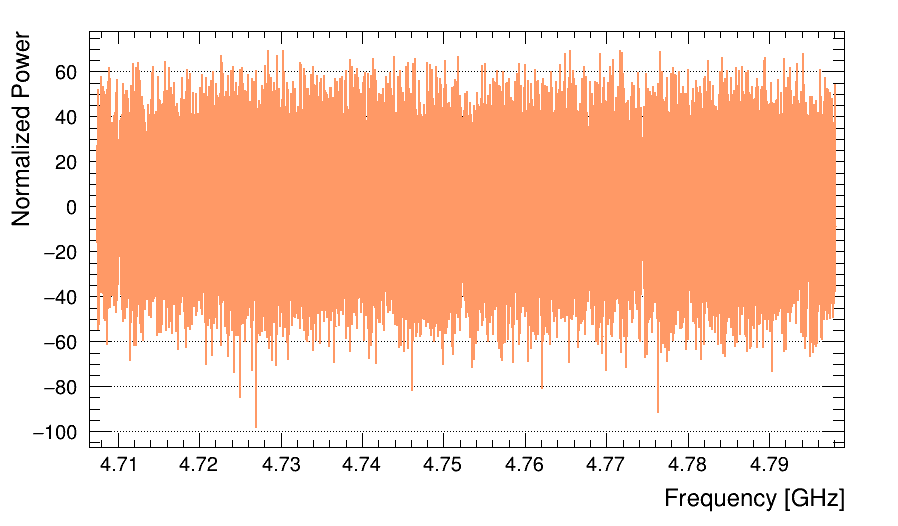
\includegraphics[width=0.4\textwidth,height = 0.3\textwidth]{figures/Power_GrandSpectrum_AxionRun_AllSteps_Rescan_Merged_5bin_SG4_W201_LqWeight.png}
    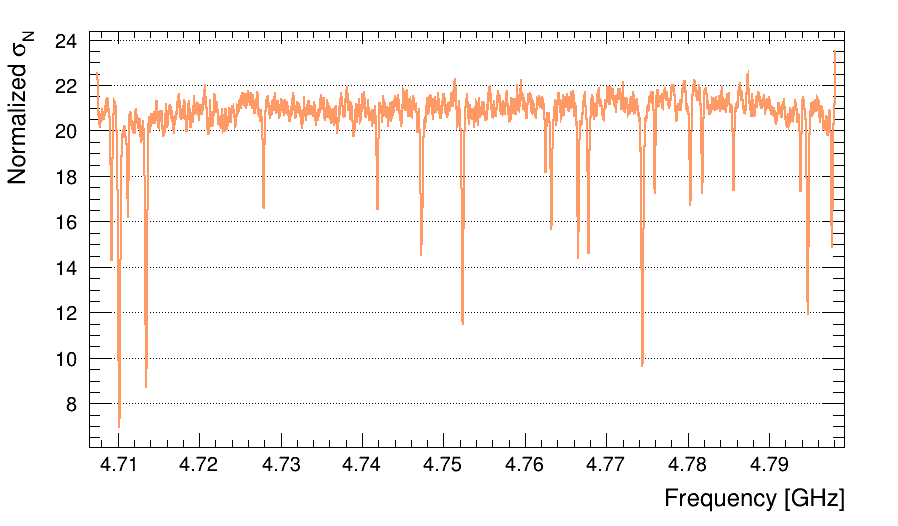
\includegraphics[width=0.4\textwidth,height = 0.3\textwidth]{figures/Sigma_GrandSpectrum_AxionRun_AllSteps_Rescan_Merged_5bin_SG4_W201_LqWeight.png}
    \caption{The merged power $\delta$ following Eq.\eqref{eq:merged_power} (left) and the standard deviation $\sigma$ derived from Eq.\eqref{eq:merged_sigma} (right)}
    \label{fig:power_sigma_merged}
\end{figure}

\begin{figure}[hbt!]
    \centering
    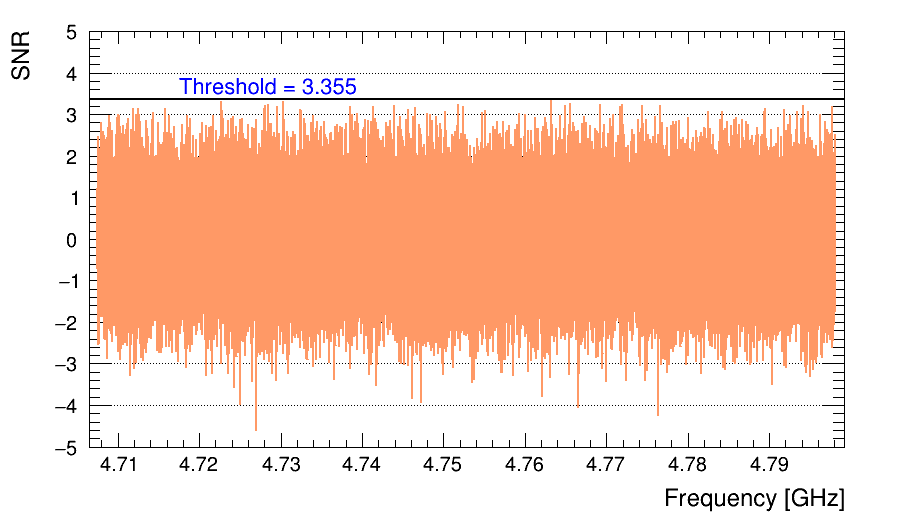
\includegraphics[width=0.8\textwidth,height=0.4\textwidth]{figures/SNR_GrandSpectrum_AxionRun_AllSteps_Rescan_Merged_5bin_SG4_W201_LqWeight.png}
    \caption{Signal-to-noise ratio (SNR) calculated using Eq.\eqref{eq:merged_snr} for merged spectrum. No candidate exceed the threshold of $3.355\sigma$ (solid-black horizontal line) }
    \label{fig:SNR_merged}
\end{figure}


After the merging, if there is any potential signal with SNR larger than 3.355 $\sigma$,
the rescan will be proceeded to check it is real signal or statistical fluctuation.
Our procedure was rescan after covering every 10 MHz range and it was done by adjusting
the tuning rod of the cavity to match the resonant frequency to the candidate.
Most of the candidates were from the fluctuations because they were gone after few rescans.
Some of them reached SNR = 3.355 $\sigma$ after rescanning, a portable antenna outside the DR was used
to probe if they came from external sources. During the data taking, several external signals from the instruments
in the laboratory were detected. More details can be found in the instrumentation paper ref~\cite{}.
